%
% .tex file needs 6_17.jpg, 6_19.jpg, and F6_26.jpg
%

\documentclass[12pt,letterpaper,boxed]{hmcpset}
\usepackage[margin=1 in]{geometry}
\usepackage{graphicx}
\usepackage{courier}
\usepackage{tabto}
\usepackage{amsmath, amssymb}
\usepackage{subfig}
\usepackage{framed}
\usepackage{enumerate}
\usepackage{pdfsync}
\usepackage{mathtools}
\usepackage{caption}
\usepackage{booktabs}
\usepackage{listings}
\usepackage{siunitx, xfrac}
\usepackage{color}



\definecolor{mygreen}{rgb}{0,0.6,0}
\definecolor{mygray}{rgb}{0.5,0.5,0.5}
\definecolor{mymauve}{rgb}{0.58,0,0.82}

\lstset{ %
  backgroundcolor=\color{white},     % choose the background color; you must add \usepackage{color} or \usepackage{xcolor}
  basicstyle=\footnotesize\ttfamily, % the size of the fonts that are used for the code
  breakatwhitespace=false,           % sets if automatic breaks should only happen at whitespace
  breaklines=true,                   % sets automatic line breaking
  captionpos=b,                      % sets the caption-position to bottom
  commentstyle=\color{mygreen},      % comment style
  deletekeywords={...},              % if you want to delete keywords from the given language
  escapeinside={\%*}{*)},            % if you want to add LaTeX within your code
  extendedchars=true,                % lets you use non-ASCII characters; for 8-bits encodings only, does not work with UTF-8
  frame=single,                      % adds a frame around the code
  keepspaces=true,                   % keeps spaces in text, useful for keeping indentation of code (possibly needs columns=flexible)
  keywordstyle=\color{blue},         % keyword style
  language=Octave,                   % the language of the code
  morekeywords={*,...},              % if you want to add more keywords to the set
  numbers=left,                      % where to put the line-numbers; possible values are (none, left, right)
  numbersep=5pt,                     % how far the line-numbers are from the code
  numberstyle=\tiny\color{mygray},   % the style that is used for the line-numbers
  rulecolor=\color{black},           % if not set, the frame-color may be changed on line-breaks within not-black text (e.g. comments (green here))
  showspaces=false,                  % show spaces everywhere adding particular underscores; it overrides 'showstringspaces'
  showstringspaces=false,            % underline spaces within strings only
  showtabs=false,                    % show tabs within strings adding particular underscores
  stepnumber=2,                      % the step between two line-numbers. If it's 1, each line will be numbered
  stringstyle=\color{mymauve},       % string literal style
  tabsize=2,                         % sets default tabsize to 2 spaces
}

\name{Jerry Hsiung}
\class{Computer Vision 16-720}
\assignment{Assignment 2}
\duedate{\today}

\begin{document}
\problemlist{Assignment \#2}

%%%%%%%%%%%%%%%%%%%%%%%%%%%%%%%%%
%		1
%%%%%%%%%%%%%%%%%%%%%%%%%%%%%%%%%



\begin{problem}[1.1]
Gaussian Pyramid of \textit{model\_chickenbroth.jpg}
\end{problem}

\begin{solution}
  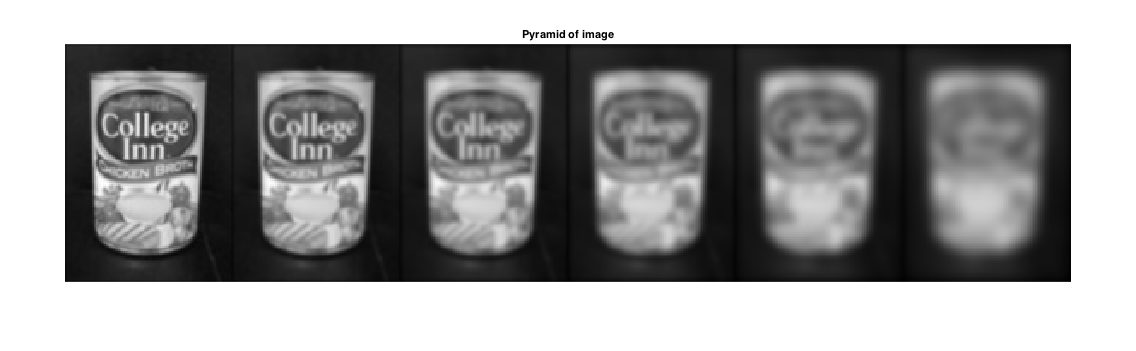
\includegraphics[width=\textwidth]{1_1.png}
\end{solution}

\begin{problem}[1.2]
Diference in Guassian Pyramid of \textit{model\_chickenbroth.jpg}

\end{problem}

\begin{solution}
  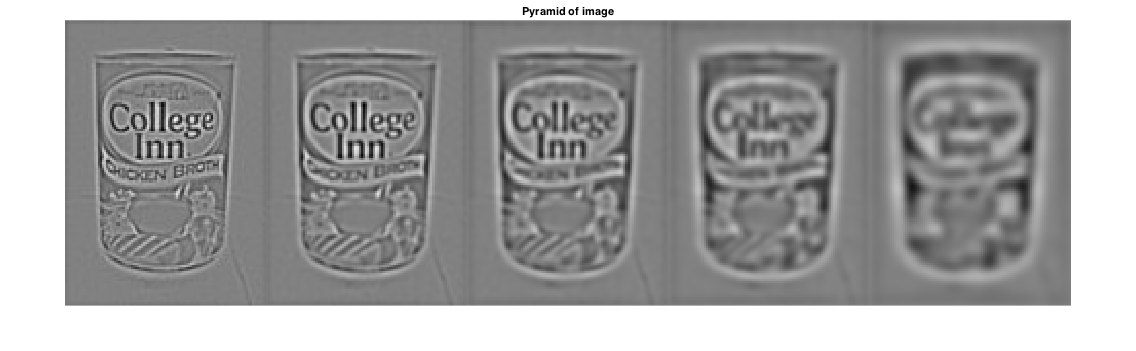
\includegraphics[width=\textwidth]{1_2.png}

\end{solution}
\newpage
\begin{problem}[1.5]
  Image of detected keypoints with edge suppresions on \textit{model\_chickenbroth.jpg}
\end{problem}

\begin{solution}
  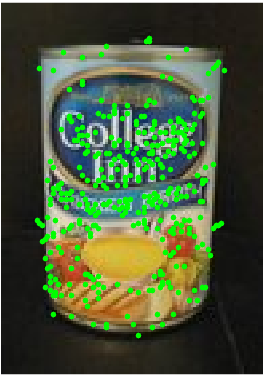
\includegraphics[width=0.5\textwidth]{1_5.png}
\end{solution}
\newpage
\begin{problem}[2.4]
  Results of two images matching on \textit{chickenbroth.jpg}, \textit{inline.jpg}, and \textit{textbook.jpg}.
\end{problem}

\begin{solution}
  The matching results are below (Running all the matching with ratio = 0.7)\\
  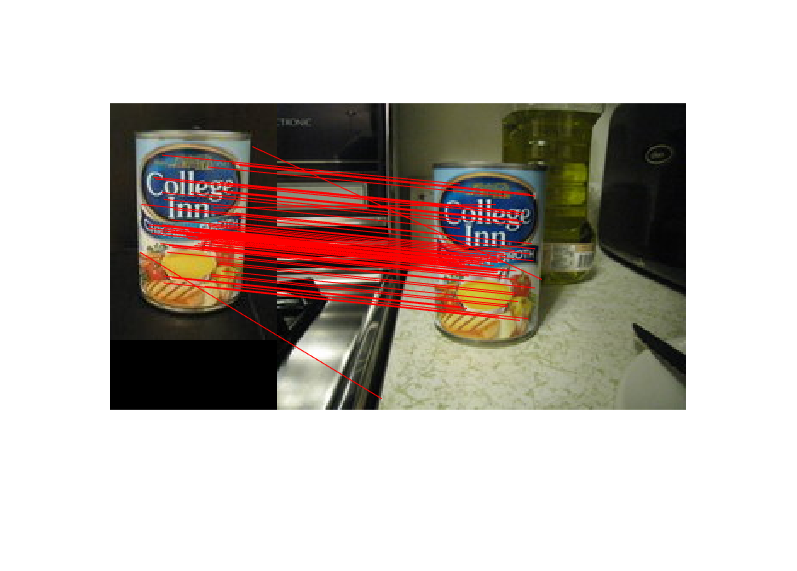
\includegraphics[width=\textwidth]{2_4_chicken.png}\\
  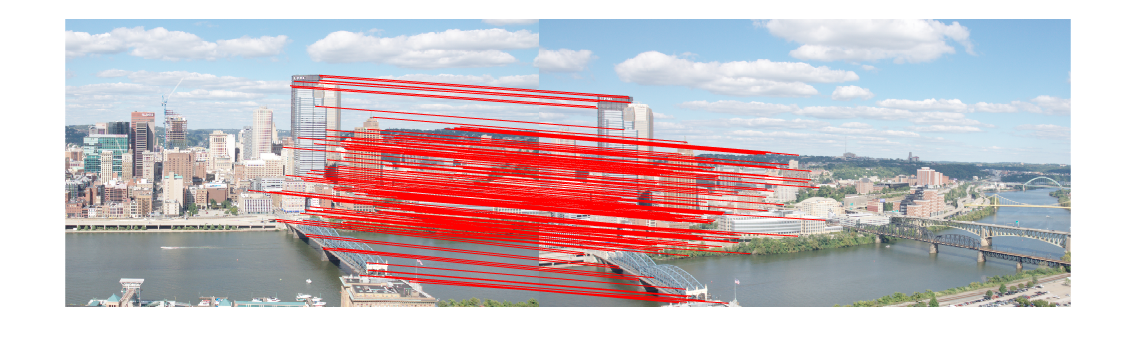
\includegraphics[width=\textwidth]{2_4_incline.png}\\
  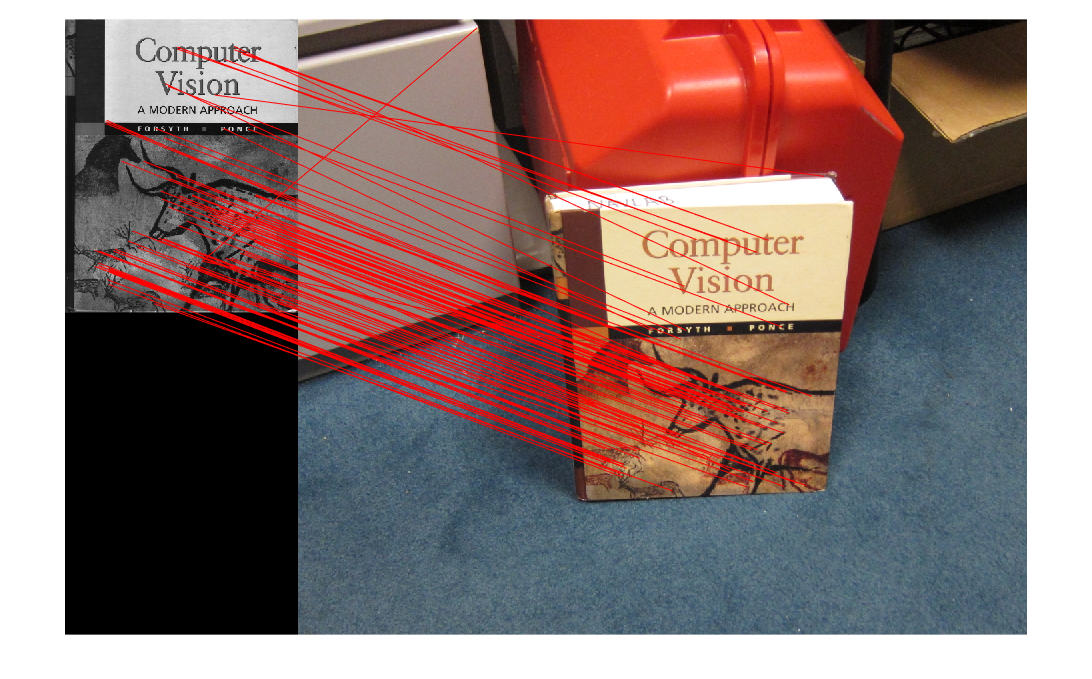
\includegraphics[width=\textwidth]{2_4_book.png}\\
  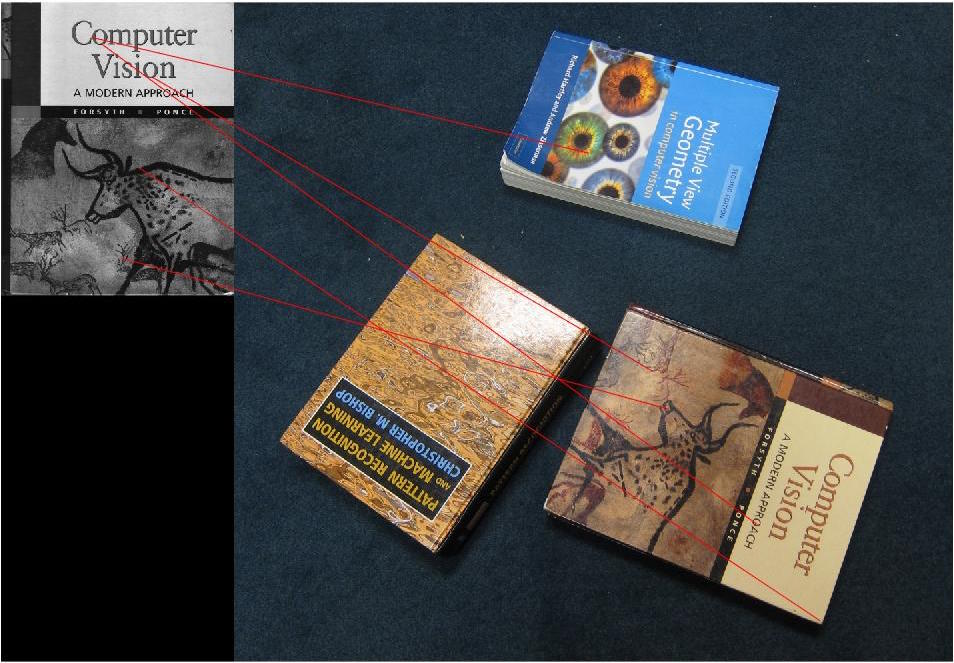
\includegraphics[width=\textwidth]{2_4_book_rot.jpg}\\
  As we can see from above, after rotation, the book is not matched well. This is because BRIEF is not
  rotation-invariant (extra credit). This is because the tests pairs that we created do not calculate 
  the same histogram after the image is rotated. One possible way to fix this is to rotate the test pairs
  too so the local environment in a descriptor will be consistent around all the interest points.
\end{solution}

\begin{problem}[2.5]
  Show the histogram of performance of matching with different rotation of \textit{model\_chickenbroth.jpg}.
\end{problem}

\begin{solution}
  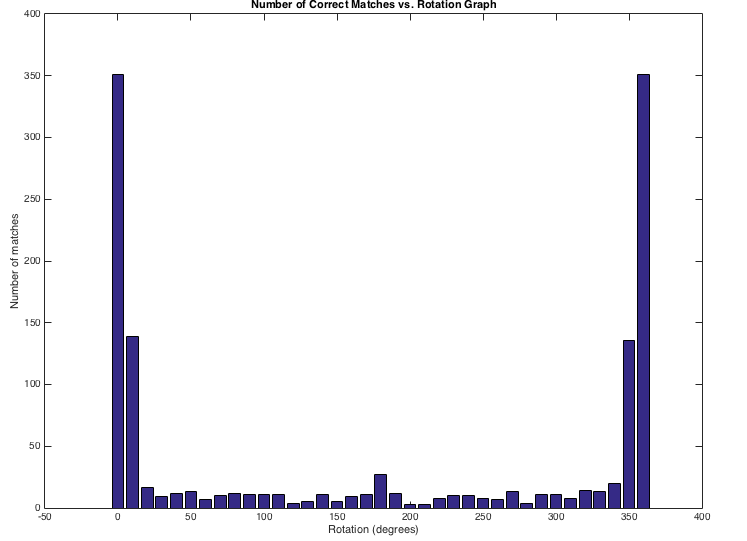
\includegraphics[width=\textwidth]{2_5.png}\\
  As discussed above (2.4), the main reason that BRIEF is not rotation invariant is because the testpairs don't 
  allow correct histogram calculation upon rotation.
\end{solution}
\newpage

\begin{problem}[3.1]
 \begin{enumerate}[(a)]
   \item Write out the expression of $\mathbf{A}$, in homography $\mathbf{Ah} = 0$.
   \item How many elements are in $\mathbf{h}$?
   \item How many point pairs (correspondences) are required to solve this system?\\
         \textit{Hint:} How many degrees of freedom are in $\mathbf{h}$? How much information does each point correspondence give?
  \item Show how to estimate the elements in $\mathbf{h}$ to find a solution to minimize this homo- geneous linear least squares system. Step us through this procedure.\\
  \textit{Hint:}  Use the Rayleigh quotient theorem (homogeneous least squares).
 \end{enumerate}
\end{problem}

\begin{solution}
\begin{enumerate}[(a)]
  \item Given that $p^i \equiv \mathbf{H}q^i$, where $p^i = [x_i', y_i', 1], q^i = [x_i, y_i,1]$, we can expand it out
  and  get the equation as:
  \begin{align*}
     \begin{pmatrix}
      x_i' \cr
      y_i' \cr
      1 \cr
      \end{pmatrix} &= \begin{pmatrix}
      h_{11} & h_{12} & h_{13}\cr
      h_{21} & h_{22} & h_{23}\cr
      h_{31} & h_{32} & h_{33}\cr
      \end{pmatrix} \begin{pmatrix}
      x_i \cr
      y_i \cr
      1 \cr
      \end{pmatrix}\\
  \end{align*}
  so divide $x_i'$ and $y_i'$ with the third row, we get:
  \begin{align*}
     \frac{x_i'}{1} &= \frac{h_{11}x_i + h_{12}y_i + h_{13}}{h_{31}x_i + h_{32}y_i + h_{33}}\\
     \frac{y_i'}{1} &= \frac{h_{21}x_i + h_{22}y_i + h_{23}}{h_{31}x_i + h_{32}y_i + h_{33}}\\
  \end{align*}
  Rearrange, we get:
  \begin{align*}
     x_i'(h_{31}x_i + h_{32}y_i + h_{33}) &= h_{11}x_i + h_{12}y_i + h_{13}\\
     h_{31}x_ix_i' + h_{32}y_i x_i'+ h_{33}x_i' -  h_{11}x_i + h_{12}y_i + h_{13} &= 0\\
     y_i'(h_{31}x_i + h_{32}y_i + h_{33}) &= h_{21}x_i + h_{22}y_i + h_{23}\\
     h_{31}x_iy_i' + h_{32}y_iy_i' + h_{33}y_i' - h_{21}x_i + h_{22}y_i + h_{23} &= 0
  \end{align*}
  Now put it in the matrix $\mathbf{Ah} = 0$, we have the desired homogeneous system for all $N$ points:
  \begin{align*}
     \begin{pmatrix}
      x_1& y_1& 1 & 0 & 0 &0&-x_1x_1'& -y_1x_1'&-x_1'\cr
      0 & 0 &0& x_1& y_1& 1 & -x_1y_1'& -y_1y_1'&-y_1'\cr
      \vdots&\vdots&\vdots&\vdots&\vdots&\vdots&\vdots&\vdots&\vdots\cr
      x_N& y_N& 1 & 0 & 0 &0&-x_Nx_N'& -y_Nx_N'&-x_N'\cr
      0 & 0 &0& x_N& y_N& 1 & -x_Ny_N'& -y_Ny_N'&-y_N'\cr
     \end{pmatrix} 
     \begin{pmatrix}
      h_{11} \cr
      h_{12} \cr
      h_{13} \cr
      h_{21} \cr
      h_{22} \cr
      h_{23} \cr
      h_{31} \cr
      h_{32} \cr
      h_{33} \cr
      \end{pmatrix} & = 0
  \end{align*}
  Now, if we have $N$ point, then the matrix $A$ will have $2N \times 9$ dimension.
  \item From above, we can see that $\mathbf{h}$ is $9\times 1$, which has 9 elements.
  \item $\mathbf{h}$ has 9 unknown, however, it is scale-invariant, which means 
  that we can multiply by a constant that eliminates one of the degree of the freedom. So $\mathbf{h}$ has 
  8 degress of freedom. Since from part (a) we see that each point provides two equations, we need a total 
  of \boxed{4} non-colinear point pairs to solve the unique system.
  \item We are trying to find $\mathbf{h}$ such that it minimizes $\mathbf{Ah}$. Using the given hint and
  Rayleigh's quotient theorem for solving homogeneous least squares (let $\mathbf{h} = x$). First we set up
  our problem as:
  \[
      argmin_{h} \frac{||Ax||^2}{||x||^2}, \text{where $||x||^2 = 1$}
  \]
  Rearrange, we get:
  \begin{align*}
   \frac{||Ax||^2}{||x||^2} = &\frac{x^TA^T Ax}{x^Tx}
  \end{align*}
  which is in Rayleigh's quotient's form. We now express $A^TA$ with its eigenvalues and eigenvectors as:
  \[
    A^TAv_i = \lambda_iv_i
  \], we can also express $x$ as the sum of on the same basis of eigenvectors $v_i$,
  \[
    x=\sum \alpha_i v_i
  \]
  So we can rewrite above as:
  \begin{align*}
   \frac{||Ax||^2}{||x||^2} &= \frac{x^TA^T Ax}{x^Tx} \\
    & = \frac{(\sum \alpha_i v_i)^TA^T A(\sum \alpha_i v_i)}{(\sum \alpha_i v_i)^T(\sum \alpha_i v_i)}\\
    & = \frac{\sum \alpha_i^2 \lambda_i}{\sum \alpha_i^2}
  \end{align*}
  Note we can simplified $v_iv_j = 0$ for $i \not = j$ because eigenvectors are orthogonal. To minimize this, we can cearly see that we want to choose the smallest
  eigenvalues $\lambda_{min}$ in $A^TA$. This is to choose $\mathbf{h}$ to be the the corresponding eigenvector in $A^TA$.
  Thus we have shown that $\mathbf{h}$ is the eigenvector corresponding to the smallest eigenvalues in $A$. (In SVD decomposition of $A = U \Sigma V^T$, this is a column of $V$ that corresponds to the smallest eighenvalues in $\Sigma$.)

\end{enumerate}
\end{solution}

\begin{problem}[5.1]
Show the warped \textit{incline\_R.png}.
\end{problem}

\begin{solution}
  below is the wraped \textit{incline\_R.png}:\\
  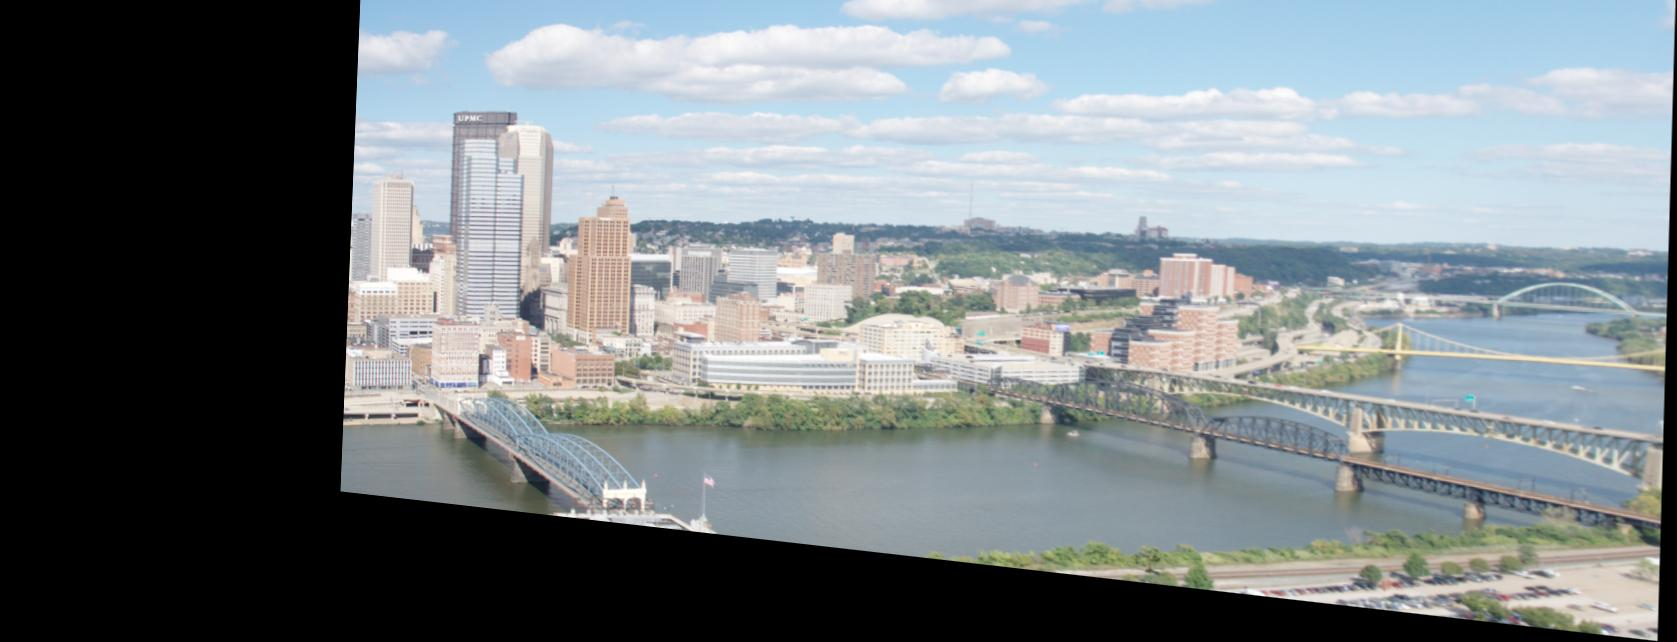
\includegraphics[width=\textwidth]{q5_1.jpg}\\
  also the stiched image:\\
    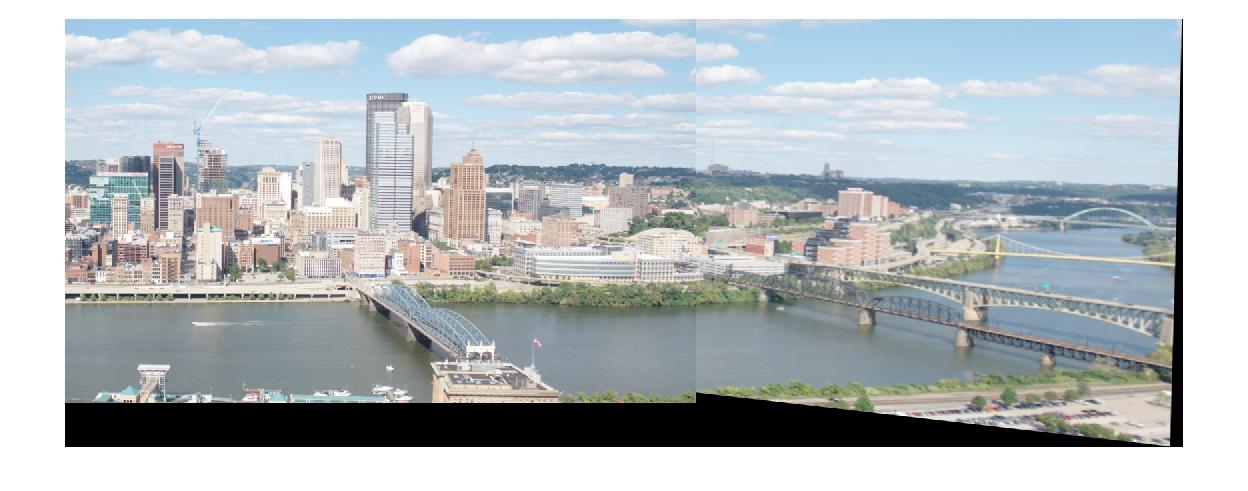
\includegraphics[width=\textwidth]{q5_1_2.jpg}\\
\end{solution}

\begin{problem}[5.2]
Show the warped \textit{incline\_R.png} with no image clipping.
\end{problem}

\begin{solution}
  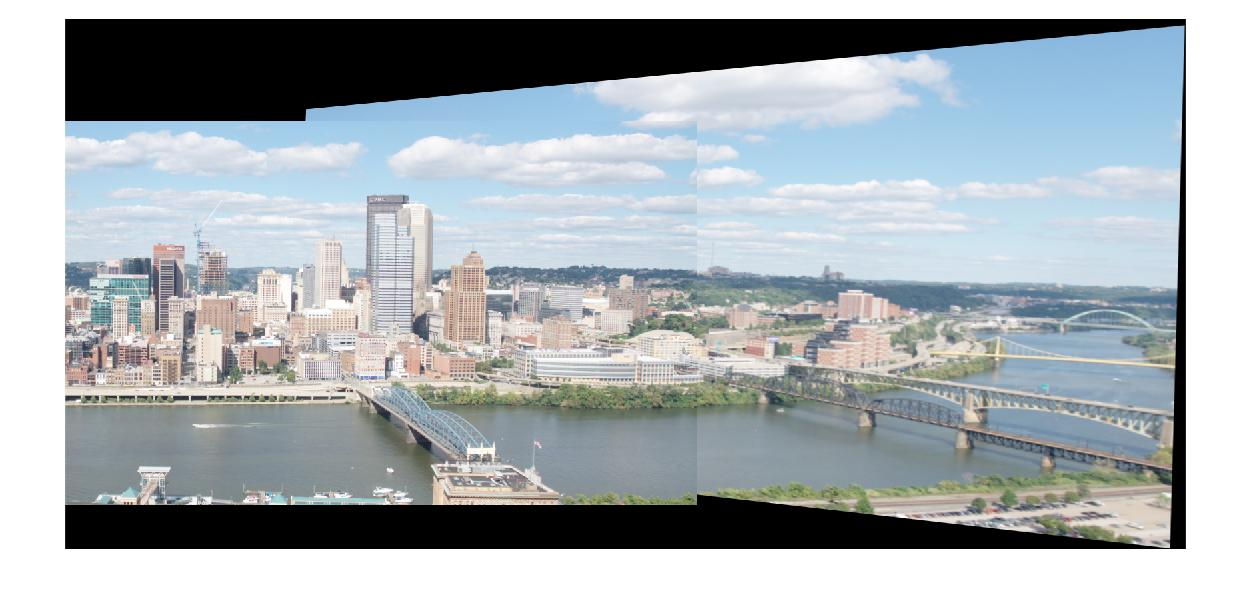
\includegraphics[width=\textwidth]{q5_2_pan.jpg}\\
\end{solution}

\begin{problem}[6.2]
Show the final panorama image with image mask blending:
\end{problem}

\begin{solution}
  The default iteration and tolerance for RANSAC are 2000 and 5:\\
  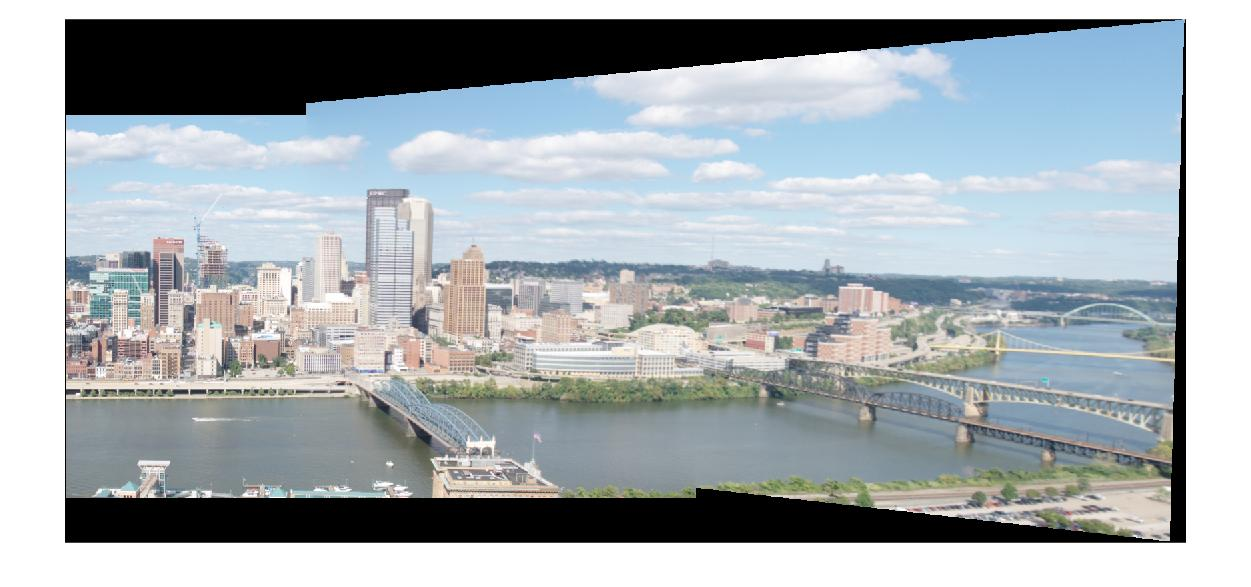
\includegraphics[width=\textwidth]{q6_2.jpg}\\
\end{solution}


\end{document}


